% Provenance (never printed): see sources/outline_sources.md (Year 1: heat sources,
% radiogenic and secular cooling; heat-flow measurement; the steady conductive geotherm
% with heat production; convection against conduction; the lithosphere as a thermal
% boundary layer). Curves from figdata/bachelor-1/geotherms.py; exercise and problem
% values in the Book 3 scratch calculator calc/ch10.py.
\chapter{Le bilan thermique de la Terre}\label{ch:b1:heat-budget}

Sous une montagne des Alpes japonaises, dans une ancienne cavité de mine, une
cuve contenant mille tonnes de scintillateur liquide guette de faibles éclairs
de lumière. La plupart proviennent d'antineutrinos produits par les réacteurs
nucléaires du pays qui l'entoure, mais certains viennent d'en bas~: l'uranium et
le thorium de la Terre émettent des antineutrinos en se désintégrant, et ceux-ci
traversent toute la planète comme si elle était vide. En 2135 jours de comptage,
le détecteur a enregistré 841 événements candidats, dont 106 ont été attribués à
la Terre elle-même. De cette poignée d'éclairs, son équipe a estimé en 2011 que
la désintégration de l'uranium et du thorium chauffe la Terre d'environ 20
térawatts. La planète entière en perd environ 47. Ce chapitre rend compte de la
différence~: d'où vient la chaleur de la Terre, comment on mesure la chaleur qui
s'en écoule, comment la température croît avec la profondeur quand la chaleur
est transportée par conduction, pourquoi le \omterm{def:b1:layered-earth:layers}{manteau} doit convecter, et pourquoi
les plaques sont la limite froide supérieure de cette convection.

\begin{recall}
La chaleur s'écoule du chaud vers le froid~; la conductivité thermique $k$ d'une
roche mesure avec quelle facilité la chaleur la traverse, sa diffusivité
thermique $\kappa = k/(\rho c)$ avec quelle rapidité une variation de température
s'y propage (physique, volume de deuxième année). Les noyaux radioactifs se
désintègrent avec une demi-vie fixe (physique). La température croît avec la
profondeur le long du \omterm{def:b1:heat-budget:geotherm}{géotherme}, et le \omterm{def:b1:layered-earth:layers}{manteau} convecte (livre~2, années~11 et~12).
La \omterm{def:b1:layered-earth:lithosphere}{lithosphère} est l'enveloppe externe résistante de la Terre
(\cref{ch:b1:layered-earth}).
\end{recall}

\section{D'où vient la chaleur}

\begin{definition}[Flux géothermique]\label{def:b1:heat-budget:heat-flow}
Le \emph{flux géothermique}\index{flux geothermique@flux géothermique} $q$ en un
point de la surface de la Terre, ou densité de flux de chaleur en surface, est la
puissance d'origine interne qui traverse la surface en ce point, par unité
d'aire, comptée positivement vers l'extérieur. Il se mesure en \unit{W.m^{-2}},
en pratique en \unit{mW.m^{-2}}. Intégré sur toute la surface, il donne la perte
de chaleur de la Terre $Q = \oint q\,\mathrm dS$.
\end{definition}

Le \omterm{def:b1:heat-budget:heat-flow}{flux géothermique} a été mesuré en des dizaines de milliers de sites. Une
compilation de \num{38347} mesures, publiée en 2010, donne les valeurs moyennes
ci-dessous, océans et continents étant comptés séparément~:
\begin{center}
\small
% ledger: dd10:split, dd10:total
\begin{tabular}{lccc}
\hline
 & aire (\unit{m^2}) & perte de chaleur (\unit{TW}) & flux moyen (\unit{mW.m^{-2}}) \\
\hline
continents & \num{2.073e14} & 14.7 & 70.9 \\
océans & \num{3.028e14} & 31.9 & 105.4 \\
Terre entière & \num{5.101e14} & 46.7 & 91.6 \\
\hline
\end{tabular}
\end{center}
Le total, arrondi à son incertitude, est $Q = \qty[uncertainty-mode=separate]{47 \pm 2}{TW}$. Les deux tiers
s'en échappent par le plancher océanique, plus jeune et plus mince que les
continents. C'est un flux faible~: le Soleil apporte environ \qty{173000}{TW} à
la Terre, et la chaleur interne ne représente que \qty{0.03}{\percent} du bilan
d'énergie en surface. % ledger: nasa:solar-mean
Mais c'est le flux qui anime les volcans, les plaques et la formation des
montagnes, et il a deux sources.

\begin{definition}[Production de chaleur radiogénique]\label{def:b1:heat-budget:heat-production}
La \emph{production de chaleur radiogénique}\index{production de chaleur radiogenique@production de chaleur radiogénique} $A$
d'une roche est la chaleur libérée par unité de volume et par unité de temps par
la désintégration des noyaux radioactifs qu'elle contient, en \unit{W.m^{-3}}, en
pratique en \unit{\micro W.m^{-3}}. Une roche de masse volumique $\rho$ contenant
les fractions massiques $C_i$ d'éléments producteurs de chaleur, chacun libérant
$H_i$ watts par kilogramme d'élément, a pour production
\[
  A = \rho \sum_i C_i H_i .
\]
\end{definition}

Quatre isotopes produisent presque toute cette chaleur, parce qu'ils ont une
longue durée de vie, une abondance suffisante et une grande énergie~:
\ce{^{238}U}, \ce{^{235}U}, \ce{^{232}Th} et \ce{^{40}K}. La chaleur par
kilogramme de chaque élément est la chaleur par kilogramme de son isotope
radioactif multipliée par la part de cet isotope dans l'élément
(\cref{exo:b1:heat-budget:3})~:
\begin{center}
\small
% ledger: dye:isotope-heat, iaea:isotopes
\begin{tabular}{lcccc}
\hline
isotope & demi-vie & chaleur par kg d'isotope & part de l'élément & chaleur par kg d'élément \\
 & (\unit{\Ga}) & (\unit{W.kg^{-1}}) & (en atomes) & (\unit{W.kg^{-1}}) \\
\hline
\ce{^{238}U} & 4.468 & \num{9.513e-5} & \qty{99.274}{\percent} & U: \num{9.85e-5} \\
\ce{^{235}U} & 0.704 & \num{5.685e-4} & \qty{0.720}{\percent} & \\
\ce{^{232}Th} & 14.0 & \num{2.628e-5} & presque tout & Th: \num{2.63e-5} \\
\ce{^{40}K} & 1.248 & \num{2.847e-5} & \qty{0.0117}{\percent} & K: \num{3.40e-9} \\
\hline
\end{tabular}
\end{center}
Le potassium libère trente mille fois moins de chaleur par kilogramme que
l'uranium, mais c'est un élément majeur de nombreuses roches, que l'on compte en
pour cent là où l'on compte l'uranium et le thorium en parties par million. Les
roches riches en ces trois éléments sont les granites et leurs apparentés~; les
plus pauvres sont les péridotites du \omterm{def:b1:layered-earth:layers}{manteau}. Une compilation de \num{2188}
analyses donne ces médianes, en \unit{\micro
W.m^{-3}}~:
\begin{center}
\small
% ledger: vila:heat-production
\begin{tabular}{lclclc}
\hline
rhyolite & 2.55 & roches argileuses & 1.44 & gabbro & 0.35 \\
granite & 2.43 & grès & 0.82 & basalte & 0.21 \\
granodiorite & 1.88 & roches carbonatées & 0.42 & roches ultramafiques & 0.11 \\
\hline
\end{tabular}
\end{center}
La dispersion dans chaque groupe est large~: un quart des granites produisent
moins de \qty{1.74}{\micro W.m^{-3}}, un quart plus de \qty{3.23}{\micro W.m^{-3}}.
La \omterm{def:b1:layered-earth:layers}{croûte} continentale est enrichie en ces éléments, la \omterm{def:b1:layered-earth:layers}{croûte} océanique et le
\omterm{def:b1:layered-earth:layers}{manteau} appauvris~; mais le \omterm{def:b1:layered-earth:layers}{manteau} est si vaste qu'il détient encore une grande
part des sources de chaleur de la planète.

\begin{definition}[Refroidissement séculaire]\label{def:b1:heat-budget:secular-cooling}
Le \emph{refroidissement séculaire}\index{refroidissement seculaire@refroidissement séculaire} est la part de la perte de
chaleur de la Terre fournie par la lente baisse de la température de son
intérieur, \omterm{def:b1:layered-earth:layers}{manteau} et noyau~: la libération de la chaleur stockée depuis la
formation de la planète, au taux $-\sum_j M_j c_j\,\mathrm dT_j/\mathrm dt$ pour
des réservoirs de masse $M_j$, de chaleur massique $c_j$ et de température
moyenne $T_j$.
\end{definition}

La conservation de l'énergie donne le bilan de la Terre entière~: la chaleur
perdue en surface est la production radiogénique plus le \omterm{def:b1:heat-budget:secular-cooling}{refroidissement séculaire},
\[
  Q = H_{\text{rad}} + Q_{\text{sc}} .
\]
Les géoneutrinos mesurent une partie du premier terme~: le résultat de 2011, qui
combinait deux détecteurs, attribue \qty{20}{TW} à l'uranium et au thorium, et
l'on sait que le \ce{^{40}K}, dont les antineutrinos sont trop faibles pour être
détectés ainsi, en ajoute environ \qty{4}{TW}.
% ledger: kamland:2011
Environ la moitié de la perte de chaleur est donc radiogénique, et l'autre moitié,
environ \qty{23}{TW}, est du \omterm{def:b1:heat-budget:secular-cooling}{refroidissement séculaire}. Une partie de ce
refroidissement est celle du noyau~: la chaleur qui traverse la \omterm{def:b1:layered-earth:discontinuity}{limite
noyau--manteau} est estimée à \qtyrange{5}{15}{TW}. Ces chiffres sont incertains~:
la mesure elle-même comporte une incertitude d'environ \qty{9}{TW}, et les
résultats des géoneutrinos ne confinent pour l'instant la part radiogénique qu'à
\qtyrange{15}{41}{TW}, tandis que les modèles de Terre de types différents
s'étalent de \qtyrange{14}{46}{TW}. Le total, mesuré en surface, est le terme le
mieux connu du bilan (figure ci-dessous).
% ledger: dye:radiogenic

\begin{omfigure}
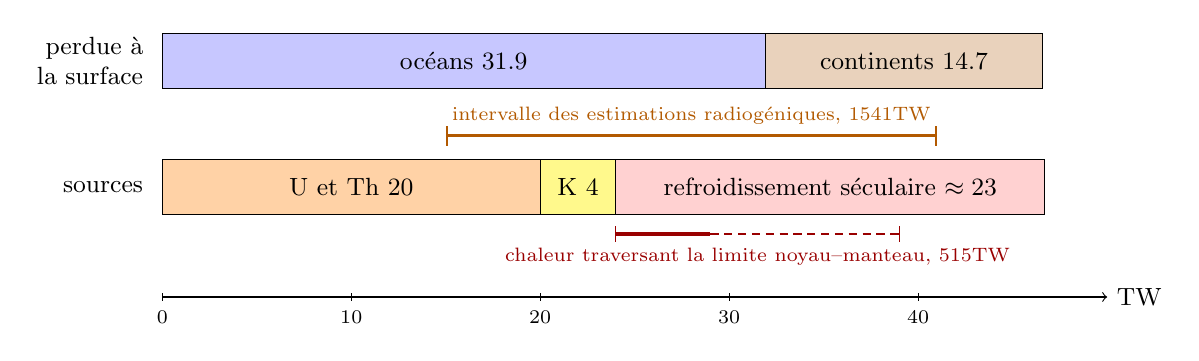
\begin{tikzpicture}[x=0.24cm, y=1cm, font=\small]
% ledger: dd10:split, kamland:2011, dye:radiogenic
% losses
\fill[blue!22] (0,1.6) rectangle (31.9,2.3);
\fill[brown!35] (31.9,1.6) rectangle (46.6,2.3);
\draw (0,1.6) rectangle (46.6,2.3);
\draw (31.9,1.6) -- (31.9,2.3);
\node at (15.95,1.95) {océans 31.9};
\node at (39.25,1.95) {continents 14.7};
\node[anchor=east, align=right, font=\small] at (-0.5,1.95) {perdue à\\la surface};
% sources
\fill[orange!35] (0,0) rectangle (20,0.7);
\fill[yellow!45] (20,0) rectangle (24,0.7);
\fill[red!18] (24,0) rectangle (46.7,0.7);
\draw (0,0) rectangle (46.7,0.7);
\draw (20,0) -- (20,0.7) (24,0) -- (24,0.7);
\node at (10,0.35) {U et Th 20};
\node at (22,0.35) {K 4};
\node at (35.35,0.35) {refroidissement séculaire $\approx 23$};
\node[anchor=east, align=right] at (-0.5,0.35) {sources};
% core part of secular cooling (range)
\draw[red!60!black, very thick] (24,-0.25) -- (29,-0.25);
\draw[red!60!black, thick, densely dashed] (29,-0.25) -- (39,-0.25);
\draw[red!60!black] (24,-0.15) -- (24,-0.35) (39,-0.15) -- (39,-0.35);
\node[anchor=north, font=\scriptsize, red!60!black] at (31.5,-0.3) {chaleur traversant la limite noyau--manteau, \qtyrange{5}{15}{TW}};
% radiogenic range
\draw[|-|, orange!70!black, thick] (15,1.0) -- (41,1.0);
\node[anchor=south, font=\scriptsize, orange!70!black] at (28,1.02) {intervalle des estimations radiogéniques, \qtyrange{15}{41}{TW}};
% axis
\draw[->] (0,-1.05) -- (50,-1.05) node[right] {TW};
\foreach \x in {0,10,20,30,40} {\draw (\x,-1.0) -- (\x,-1.1) node[below, font=\scriptsize] {\x};}
\end{tikzpicture}

\par\smallskip{\small Le bilan thermique de la Terre. En haut~: la chaleur perdue par
le plancher océanique et par les continents, \qty[uncertainty-mode=separate]{47 \pm 2}{TW} au total. En bas~: ses sources,
avec la part radiogénique de l'uranium et du thorium mesurée par les géoneutrinos et
celle du potassium estimée~; le reste, par différence, est le \omterm{def:b1:heat-budget:secular-cooling}{refroidissement
séculaire}, dont le noyau fournit une part mal connue. La barre orange montre
l'intervalle de la part radiogénique permis par les mesures de géoneutrinos.}
\label{fig:b1:heat-budget:budget}
\end{omfigure}

La chaleur radiogénique était plus grande dans le passé, parce que les isotopes
étaient plus abondants~: le \ce{^{235}U} et le \ce{^{40}K}, ceux de courte
durée de vie, contribuaient alors bien davantage (livre~2, année~12). Le moteur
thermique de la Terre ralentit lentement, sur les deux tableaux.

\section{Mesurer le flux géothermique}

Le \omterm{def:b1:heat-budget:heat-flow}{flux géothermique} ne se mesure pas directement~: on le calcule à partir d'un
gradient de température et d'une conductivité.

\begin{proposition}[Loi de Fourier]\label{prop:b1:heat-budget:fourier}
Dans un milieu de conductivité thermique $k$, la chaleur est conduite le long du
gradient de température à un taux par unité d'aire qui lui est proportionnel. Avec
$z$ la profondeur, comptée positivement vers le bas, et $q$ compté positivement
vers le haut,
\[
  q = k\,\frac{\mathrm dT}{\mathrm dz} .
\]
\end{proposition}
\admitted

La loi est établie dans le volume de deuxième année des livres de physique. La
plupart des roches conduisent la chaleur à \qtyrange{1.5}{3}{W.m^{-1}.K^{-1}} en
dessous de \qty{200}{\celsius}, moins quand elles sont chaudes~; les modèles du
flux continental donnent à la \omterm{def:b1:layered-earth:layers}{croûte} supérieure granitique environ
\qty{2.7}{W.m^{-1}.K^{-1}}~;
% ledger: delaney:conductivity, roy:granitic-k
un gradient de \qty{25}{K.km^{-1}} y signifie un flux d'environ
\qty{70}{mW.m^{-2}}.

Quand les roches traversées par un forage ont des conductivités différentes, le
gradient change de l'une à l'autre, mais pas le flux, tant qu'aucune chaleur
n'est produite ni stockée entre elles. La proposition suivante en fait un test.

\begin{proposition}[Diagramme de Bullard]\label{prop:b1:heat-budget:bullard}
Soit $R(z) = \int_0^z \mathrm d\zeta/k(\zeta)$ la résistance thermique, par unité
d'aire, des roches comprises entre la surface et la profondeur $z$, en
\unit{m^2.K.W^{-1}}. Si le flux $q$ est le même à toute profondeur d'un forage,
la température est une fonction linéaire de la résistance thermique~:
$T(z) = T_0 + q\,R(z)$.
\end{proposition}

\begin{proof}
D'après la loi de Fourier, $\mathrm dT/\mathrm dz = q/k(z)$. En intégrant de $0$ à
$z$ avec $q$ constant, $T(z) - T_0 = q\int_0^z \mathrm d\zeta/k(\zeta) = q\,R(z)$.
\end{proof}

\begin{method}[Le flux géothermique à partir d'un forage]\label{met:b1:heat-budget:borehole}
\begin{enumerate}
  \item Enregistrer la température le long du forage longtemps après le forage,
        quand la perturbation due au fluide de forage s'est éteinte, et mettre de
        côté les quelques dizaines de mètres les plus proches de la surface, qui
        suivent les saisons.
  \item Mesurer au laboratoire la conductivité d'échantillons carottés de chaque
        roche traversée, et calculer la résistance thermique $R(z)$ à chaque
        profondeur enregistrée.
  \item Tracer $T$ en fonction de $R$~: la pente de la droite est le \omterm{def:b1:heat-budget:heat-flow}{flux
        géothermique}. Une cassure révèle de l'eau circulant dans les roches, un
        changement passé de la température de surface, ou une erreur sur une
        conductivité.
  \item Corriger, si besoin, du relief, qui courbe les isothermes sous les
        collines et les vallées, et du lent réchauffement depuis la dernière
        glaciation, qui perturbe encore le premier kilomètre environ.
\end{enumerate}
\end{method}

En mer, il n'est pas besoin de forage. La température au fond de l'océan profond
est très stable, si bien que quelques mètres de sédiment meuble portent déjà le
gradient d'équilibre. Une lance d'acier portant une rangée de capteurs de
température est larguée d'un navire et enfoncée dans le sédiment par un lourd
poids (figure ci-dessous)~; les capteurs enregistrent le gradient, et une
impulsion de chaleur envoyée le long de la lance donne la conductivité du
sédiment en place.
Le plancher océanique a un piège. Sur la \omterm{def:b1:layered-earth:layers}{croûte} jeune, l'eau de mer circule à
travers le basalte fissuré et emporte une bonne part de la chaleur par advection,
si bien que le flux conductif mesuré est bien en deçà de la perte réelle. La perte
à travers le plancher le plus jeune est donc calculée à partir du modèle de
refroidissement de la \cref{sec:b1:heat-budget:boundary-layer}, calé sur la
\omterm{def:b1:layered-earth:layers}{croûte} ancienne où la circulation a cessé~: cette part calculée, \qty{23.1}{TW},
fait environ la moitié du total mondial. % ledger: dd10:young-ocean

\begin{omfigure}
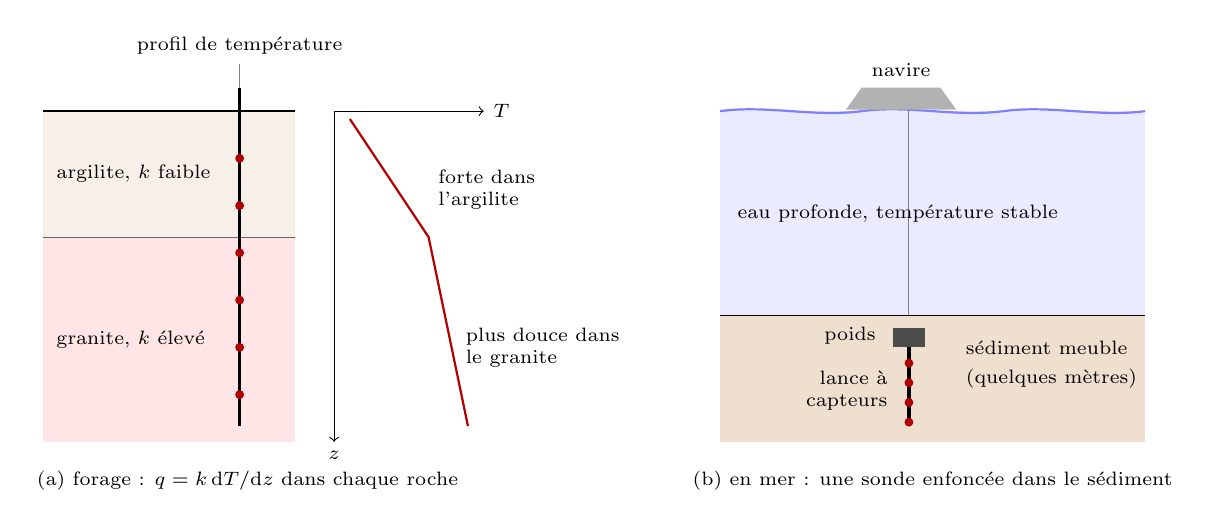
\begin{tikzpicture}[font=\scriptsize, x=1cm, y=1cm]
% --- left: borehole on land ---
\fill[brown!12] (0,0) rectangle (3.2,-1.6);
\fill[red!10] (0,-1.6) rectangle (3.2,-4.2);
\draw[thick] (0,0) -- (3.2,0);
\node[anchor=west] at (0.05,-0.8) {argilite, $k$ faible};
\node[anchor=west] at (0.05,-2.9) {granite, $k$ élevé};
\draw[black!60] (0,-1.6) -- (3.2,-1.6);
\draw[very thick] (2.5,0.3) -- (2.5,-4.0);
\draw[gray] (2.5,0.6) -- (2.5,0.3);
\foreach \y in {-0.6,-1.2,-1.8,-2.4,-3.0,-3.6} {\fill[red!70!black] (2.5,\y) circle (1.6pt);}
\node[anchor=south] at (2.5,0.6) {profil de température};
% inset T(z)
\draw[->] (3.7,0) -- (5.6,0) node[right] {$T$};
\draw[->] (3.7,0) -- (3.7,-4.2) node[below] {$z$};
\draw[thick, red!70!black] (3.9,-0.1) -- (4.9,-1.6) -- (5.4,-4.0);
\node[anchor=west, align=left] at (4.9,-1.0) {forte dans\\l'argilite};
\node[anchor=west, align=left] at (5.25,-3.0) {plus douce dans\\le granite};
\node[anchor=north] at (2.6,-4.45) {(a) forage~: $q = k\,\mathrm dT/\mathrm dz$ dans chaque roche};
% --- right: probe at sea ---
\begin{scope}[xshift=8.6cm]
\fill[blue!8] (0,0) rectangle (5.4,-2.6);
\draw[blue!50, thick] (0,0) .. controls (0.6,0.08) and (1.2,-0.08) .. (1.8,0)
  .. controls (2.4,0.08) and (3.0,-0.08) .. (3.6,0) .. controls (4.2,0.08) and (4.8,-0.08) .. (5.4,0);
\fill[gray!60] (1.6,0.02) -- (3.0,0.02) -- (2.8,0.3) -- (1.8,0.3) -- cycle;
\node[anchor=south] at (2.3,0.32) {navire};
\draw[gray] (2.4,0.02) -- (2.4,-2.75);
\fill[brown!25] (0,-2.6) rectangle (5.4,-4.2);
\draw (0,-2.6) -- (5.4,-2.6);
\node[anchor=west] at (3.0,-3.0) {sédiment meuble};
\node[anchor=west] at (3.0,-3.4) {(quelques mètres)};
\fill[black!70] (2.2,-2.75) rectangle (2.6,-3.0);
\draw[very thick] (2.4,-3.0) -- (2.4,-4.0);
\foreach \y in {-3.2,-3.45,-3.7,-3.95} {\fill[red!70!black] (2.4,\y) circle (1.6pt);}
\node[anchor=east, align=right] at (2.1,-2.85) {poids};
\node[anchor=east, align=right] at (2.25,-3.55) {lance à\\capteurs};
\node[anchor=west] at (0.1,-1.3) {eau profonde, température stable};
\node[anchor=north] at (2.7,-4.45) {(b) en mer~: une sonde enfoncée dans le sédiment};
\end{scope}
\end{tikzpicture}

\par\smallskip{\small Mesurer le \omterm{def:b1:heat-budget:heat-flow}{flux géothermique} (schéma, hors échelle). (a) À
terre, la température est enregistrée le long d'un forage une fois revenue à
l'équilibre, et la conductivité de chaque roche est mesurée sur des carottes~: le
gradient est plus fort là où la conductivité est plus faible, et le flux, leur
produit, est le même. (b) En mer, une lance à capteurs est enfoncée de quelques
mètres dans le sédiment du plancher océanique.}
\label{fig:b1:heat-budget:measure}
\end{omfigure}

\begin{inthefield}[Le flux géothermique en mer]
\begin{minipage}[t]{0.55\linewidth}\vspace{0pt}
Sur un navire de recherche, la sonde de flux est une lourde lance suspendue à la
grue de poupe. On la descend au bout du câble du navire jusque juste au-dessus du
fond marin, puis on la lâche~: le poids l'enfonce dans le sédiment, et l'équipage
attend sur le pont que les capteurs se mettent à la température de la vase, puis
la remonte et passe à la station suivante, un peu plus loin. Une ligne de telles
stations à travers le flanc d'une dorsale donne la décroissance du flux avec
l'âge du plancher, et la dispersion entre stations voisines montre où l'eau
circule à travers la \omterm{def:b1:layered-earth:layers}{croûte} en dessous.
\end{minipage}\hfill
\begin{minipage}[t]{0.42\linewidth}\vspace{0pt}
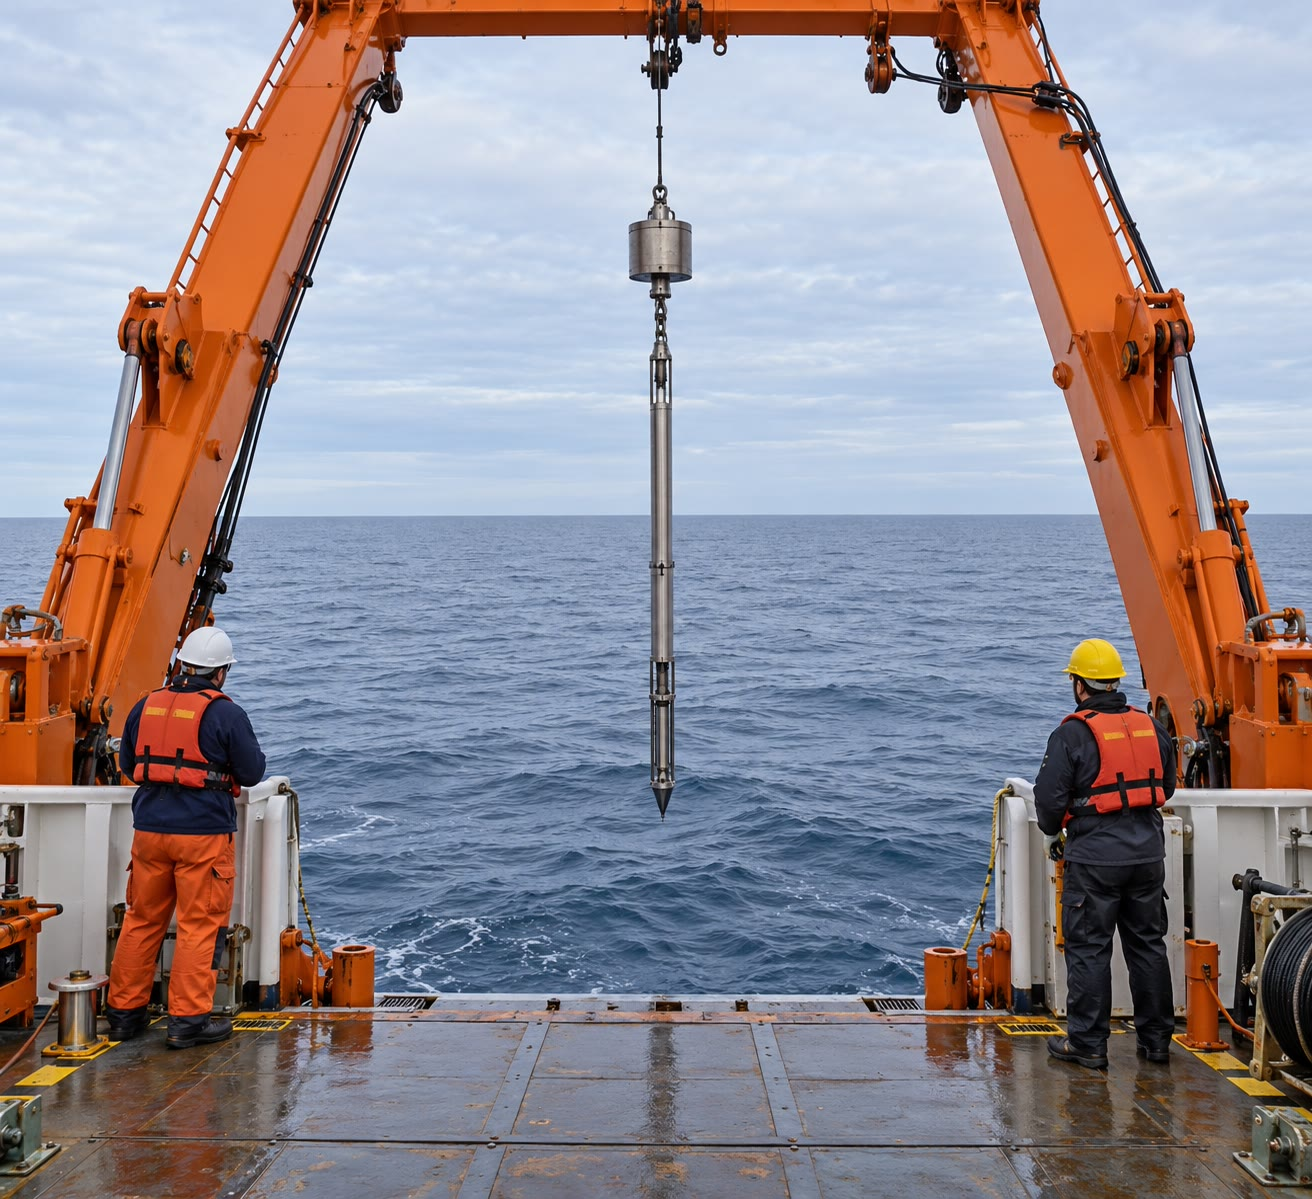
\includegraphics[width=\linewidth]{images/book3/ai/b1-heatflow-probe.jpg}

{\scriptsize Une sonde de \omterm{def:b1:heat-budget:heat-flow}{flux géothermique} suspendue à la grue de poupe d'un
navire de recherche (illustration générée par IA).}
\end{minipage}
\end{inthefield}

\section{Le géotherme conductif stationnaire}

\begin{definition}[Géotherme]\label{def:b1:heat-budget:geotherm}
Le \emph{géotherme}\index{geotherme@géotherme} sous un point de la surface est la
température en fonction de la profondeur en ce point, $T(z)$. C'est un
géotherme conductif stationnaire lorsqu'il ne change pas avec le temps et que la
chaleur y est transportée par conduction seule.
\end{definition}

Dans la \omterm{def:b1:layered-earth:lithosphere}{lithosphère}, loin des volcans actifs et de la circulation d'eau, la
chaleur est transportée par conduction, et à l'échelle de millions d'années le
\omterm{def:b1:heat-budget:geotherm}{géotherme} est stationnaire. Sa forme découle alors d'un bilan d'énergie.

\begin{theorem}[Conduction stationnaire avec production de chaleur]\label{thm:b1:heat-budget:balance}
Le long d'un \omterm{def:b1:heat-budget:geotherm}{géotherme} conductif stationnaire, dans un milieu de conductivité
uniforme $k$ avec une production de chaleur $A(z)$ et sans flux horizontal de
chaleur,
\[
  \frac{\mathrm dq}{\mathrm dz} = -A(z), \qquad\text{c'est-à-dire}\qquad
  k\,\frac{\mathrm d^2T}{\mathrm dz^2} = -A(z).
\]
\end{theorem}

\begin{proof}
Considérons une tranche horizontale d'aire $S$ entre les profondeurs $z$ et $z +
\mathrm dz$. La chaleur entre par sa base au taux $q(z + \mathrm dz)\,S$, sort
par son sommet au taux $q(z)\,S$, et est produite à l'intérieur au taux
$A(z)\,S\,\mathrm dz$. En régime stationnaire aucune chaleur n'est stockée, donc
$q(z)\,S = q(z + \mathrm dz)\,S + A(z)\,S\,\mathrm dz$, ce qui donne
$\mathrm dq/\mathrm dz = -A$. D'après la loi de Fourier $q = k\,\mathrm dT/\mathrm dz$,
et avec $k$ uniforme, $k\,T'' = -A$.
\end{proof}

En lisant de la surface vers le bas, le flux décroît avec la profondeur de la
chaleur produite au-dessus de chaque niveau~: ce qui traverse la surface est la
chaleur venue d'en dessous plus toute la chaleur produite en chemin. Deux
distributions de $A$ donnent des formes fermées.

\begin{proposition}[Une couche radiogénique uniforme]\label{prop:b1:heat-budget:uniform}
Soit une production de chaleur $A$ de la surface jusqu'à la profondeur $h$ et
nulle en dessous, la surface à la température $T_0$ et le flux de surface $q_0$.
Alors pour $0 \le z \le h$
\[
  q(z) = q_0 - A z, \qquad T(z) = T_0 + \frac{q_0 z}{k} - \frac{A z^2}{2k},
\]
et au-dessous de $h$ le flux est uniforme, $q_m = q_0 - A h$, et le \omterm{def:b1:heat-budget:geotherm}{géotherme} une
droite de pente $q_m/k$.
\end{proposition}

\begin{proof}
Intégrer $\mathrm dq/\mathrm dz = -A$ à partir de $0$ avec $q(0) = q_0$~: $q = q_0 -
Az$. Puis $\mathrm dT/\mathrm dz = (q_0 - Az)/k$~; en intégrant avec $T(0) = T_0$
on obtient la parabole. Au-dessous de $h$, $\mathrm dq/\mathrm dz = 0$ et $q$
garde sa valeur en $h$.
\end{proof}

\begin{theorem}[Production de chaleur exponentielle et relation linéaire du flux]
\label{thm:b1:heat-budget:exponential}
Soit une production de chaleur qui décroît avec la profondeur comme $A(z) = A_0 e^{-z/D}$,
un flux qui tend vers $q_m$ à grande profondeur, et la surface à $T_0$. Alors
\[
  q(z) = q_m + A_0 D\,e^{-z/D}, \qquad
  T(z) = T_0 + \frac{q_m z}{k} + \frac{A_0 D^2}{k}\bigl(1 - e^{-z/D}\bigr),
\]
et le flux de surface est
\[
  q_0 = q_m + A_0 D .
\]
\end{theorem}

\begin{proof}
D'après le \cref{thm:b1:heat-budget:balance}, $\mathrm dq/\mathrm dz =
-A_0e^{-z/D}$, donc $q(z) = A_0 D e^{-z/D} + C$~; quand $z \to \infty$, $q \to C$,
d'où $C = q_m$. En $z = 0$, $q_0 = q_m + A_0 D$. Puis $\mathrm dT/\mathrm dz =
q/k = q_m/k + (A_0D/k)\,e^{-z/D}$, et en intégrant à partir de $0$ avec $T(0) = T_0$,
$T = T_0 + q_m z/k + (A_0 D^2/k)(1 - e^{-z/D})$.
\end{proof}

La dernière ligne est une prédiction que l'on peut tester en surface. Des plutons
granitiques d'une même région partagent le même flux profond $q_m$ et, s'ils ne
diffèrent que par leur richesse en uranium, thorium et potassium, la même échelle
$D$~; alors le flux mesuré au-dessus de chaque pluton doit être une fonction
linéaire de la production de chaleur mesurée sur ses roches, de pente $D$, une
longueur, et d'ordonnée à l'origine $q_m$, le flux réduit, venant de
dessous la couche radiogénique. Francis Birch observa le premier une telle droite,
rapportée en 1968, et la même année trois provinces furent définies par leurs
droites~:
\begin{center}
\small
% ledger: roy:provinces, roy:linear-relation
\begin{tabular}{lcc}
\hline
province & ordonnée à l'origine $q_m$ (\unit{mW.m^{-2}}) & pente $D$ (\unit{km}) \\
\hline
est des États-Unis & 33 & 7.5 \\
Basin and Range (Grand Bassin) & 59 & 9.4 \\
Sierra Nevada & 17 & 10 \\
\hline
\end{tabular}
\end{center}
Les ordonnées à l'origine, publiées sous la forme 0.8, 1.4 et $0.4\times\qty{e-6}{cal.cm^{-2}.s^{-1}}$,
sont converties avec $\qty{1}{\micro cal.cm^{-2}.s^{-1}} = \qty{41.84}{mW.m^{-2}}$
(\cref{exo:b1:heat-budget:4}). Les pentes varient peu, de 7 à \qty{10}{km}~; le flux
réduit varie beaucoup, et ses cartes montrent où le \omterm{def:b1:layered-earth:layers}{manteau} en dessous est chaud,
comme sous la \omterm{def:b1:layered-earth:layers}{croûte} étirée du Basin and Range. La couche uniforme de
la \cref{prop:b1:heat-budget:uniform} donne aussi une droite, de pente $h$~:
les deux modèles s'ajustent aux données, mais seul l'exponentiel reste une droite
de même pente quand les plutons sont érodés à des profondeurs différentes
(\cref{exo:b1:heat-budget:10}), ce qui le fait préférer.

\begin{omfigure}
\begin{tikzpicture}
\begin{axis}[omdepth, width=0.82\linewidth, height=8.6cm, xmin=0, xmax=1800, ymin=0, ymax=250, axis x line=top, axis y line=left, axis line style={-}, clip=true,
  xlabel={température (\unit{\degreeCelsius})}, ylabel={profondeur (km)},
  tick label style={font=\scriptsize}, label style={font=\small},
  legend style={font=\scriptsize, at={(0.02,0.02)}, anchor=south west, draw=none, fill=white, fill opacity=0.85, text opacity=1},
  legend cell align=left]
\addplot[very thick, black!45] table[x=T, y=depth] {figdata/out/bachelor-1-geotherms-adiabat.dat};
\addlegendentry{adiabate du manteau}
\addplot[very thick, red!75!black] table[x=T45, y=depth] {figdata/out/bachelor-1-geotherms-continental.dat};
\addlegendentry{$q_0 = \qty{70}{mW.m^{-2}}$}
\addplot[very thick, orange!80!black] table[x=T30, y=depth] {figdata/out/bachelor-1-geotherms-continental.dat};
\addlegendentry{$q_0 = \qty{55}{mW.m^{-2}}$}
\addplot[very thick, green!45!black] table[x=T15, y=depth] {figdata/out/bachelor-1-geotherms-continental.dat};
\addlegendentry{$q_0 = \qty{40}{mW.m^{-2}}$}
\addplot[thick, blue!70!black, densely dashdotted] table[x=T, y=depth] {figdata/out/bachelor-1-geotherms-oceanic.dat};
\addlegendentry{plancher océanique de \qty{60}{\Ma}}
\addplot[thin, dashed, red!75!black, forget plot] table[x=Tc45, y=depth] {figdata/out/bachelor-1-geotherms-continental.dat};
\addplot[thin, dashed, orange!80!black, forget plot] table[x=Tc30, y=depth] {figdata/out/bachelor-1-geotherms-continental.dat};
\addplot[thin, dashed, green!45!black, forget plot] table[x=Tc15, y=depth] {figdata/out/bachelor-1-geotherms-continental.dat};
\draw[densely dotted, black!60] (axis cs:0,35) -- (axis cs:1800,35);
\node[font=\scriptsize, anchor=south east] at (axis cs:1790,35) {Moho, \qty{35}{km}};
\fill (axis cs:1384.0,70.8) circle (1.6pt);
\fill (axis cs:1403.2,107.8) circle (1.6pt);
\fill (axis cs:1459.7,224.9) circle (1.6pt);
\node[font=\scriptsize, anchor=west] at (axis cs:1420,66) {\qty{71}{km}};
\node[font=\scriptsize, anchor=west] at (axis cs:1440,104) {\qty{108}{km}};
\node[font=\scriptsize, anchor=west] at (axis cs:1495,222) {\qty{225}{km}};
\end{axis}
\end{tikzpicture}

\par\smallskip{\small \omterm{def:b1:heat-budget:geotherm}{Géothermes} conductifs stationnaires d'un continent dont la
production de chaleur $A_0 = \qty{2.5}{\micro W.m^{-3}}$ décroît sur $D = \qty{10}{km}$,
$k = \qty{2.5}{W.m^{-1}.K^{-1}}$, pour trois flux de surface (flux réduit
15, 30 et \qty{45}{mW.m^{-2}}). Chacun suit sa courbe conductive (en tirets
au-delà) jusqu'à l'\omterm{def:b1:heat-budget:adiabat}{adiabate du manteau}, qu'il rejoint au point~: la base de la
\omterm{def:b1:heat-budget:boundary-layer}{lithosphère thermique}. Le \omterm{def:b1:heat-budget:geotherm}{géotherme} du plancher océanique est celui d'un demi-espace refroidi pendant
\qty{60}{\Ma}. La conductivité uniforme est une simplification.}
\label{fig:b1:heat-budget:geotherms}
\end{omfigure}

\begin{method}[La température en profondeur sous un pluton]\label{met:b1:heat-budget:moho}
\begin{enumerate}
  \item Mesurer le flux de surface $q_0$ au-dessus du pluton (méthode du forage)
        et sa production de chaleur $A_0$ d'après ses teneurs en U, Th et K.
  \item À partir de la droite de la province, ou avec une valeur de $D$
        d'environ \qty{10}{km}, calculer $q_m = q_0 - A_0 D$.
  \item Appliquer le \cref{thm:b1:heat-budget:exponential}. Au-delà de quelques fois $D$,
        $e^{-z/D}$ est négligeable et le \omterm{def:b1:heat-budget:geotherm}{géotherme} est la droite
        $T_0 + A_0D^2/k + q_m z/k$~: la couche radiogénique a élevé toutes les
        températures profondes de $A_0D^2/k$.
\end{enumerate}
\end{method}

Sur la figure, la température au \omterm{def:b1:layered-earth:discontinuity}{Moho} va d'environ \qty{320}{\degreeCelsius}
pour le flux le plus faible à plus de \qty{700}{\degreeCelsius} pour le plus fort~: le \omterm{def:b1:heat-budget:heat-flow}{flux
géothermique} de surface porte une lecture directe de la
température de la \omterm{def:b1:layered-earth:layers}{croûte} profonde, qui gouverne sa résistance
(\cref{ch:b1:stress-strain-rheology}).

\section{Conduction contre convection}

La conduction est lente. À quel point, l'équation de la chaleur le dit~; les
livres de physique la déduisent de la loi de Fourier et du bilan du
\cref{thm:b1:heat-budget:balance} complété par le stockage~: en une dimension,
sans production de chaleur,
$\partial T/\partial t = \kappa\,\partial^2 T/\partial z^2$.

\begin{proposition}[L'échelle de temps conductive]\label{prop:b1:heat-budget:timescale}
Une variation de température imposée à la frontière d'un corps conducteur se
propage sur une distance $L$ en un temps de l'ordre de
\[
  \tau = \frac{L^2}{\kappa} .
\]
\end{proposition}

\begin{proof}
Écrivons $z = L z^*$, $t = \tau t^*$, avec $z^*$ et $t^*$ sans dimension. L'équation
de la chaleur devient $\partial T/\partial t^* = (\kappa\tau/L^2)\,\partial^2
T/\partial z^{*2}$. Ses solutions varient à l'échelle $z^* \sim 1$ quand $t^* \sim 1$
seulement si le coefficient est d'ordre un, c'est-à-dire si $\tau \sim L^2/\kappa$.
\end{proof}

Les roches ont $\kappa \approx \qty{e-6}{m^2.s^{-1}}$. Le cycle journalier de
température pénètre de quelques dizaines de centimètres dans le sol, le cycle
annuel de quelques mètres, et le réchauffement depuis la dernière glaciation d'un
kilomètre environ. À travers une \omterm{def:b1:layered-earth:lithosphere}{lithosphère} épaisse de \qty{100}{km},
$\tau = \qty{e16}{s}$, soit environ \qty{300}{\Ma}. À travers le \omterm{def:b1:layered-earth:layers}{manteau}, épais de
\qty{2900}{km}, $\tau = \qty{8.4e18}{s}$, soit \qty{270}{\Ga}~: soixante fois
l'âge de la Terre, \qty{4.54}{\Ga}. % ledger: england:kelvin, usgs:age-earth
La conduction seule n'aurait pu amener la chaleur du \omterm{def:b1:layered-earth:layers}{manteau} profond nulle part
près de la surface. Le \omterm{def:b1:layered-earth:layers}{manteau} convecte, et dans son intérieur la chaleur est
transportée par le mouvement de la roche elle-même, à la vitesse des plaques, des
centimètres par an. % ledger: usgs:san-andreas

\begin{definition}[Adiabate du manteau]\label{def:b1:heat-budget:adiabat}
L'\emph{adiabate du manteau}\index{adiabate du manteau} est le \omterm{def:b1:heat-budget:geotherm}{géotherme} de
l'intérieur bien mélangé du \omterm{def:b1:layered-earth:layers}{manteau} en convection~: la température que prend la
roche du \omterm{def:b1:layered-earth:layers}{manteau} quand elle monte ou descend assez vite pour n'échanger aucune
chaleur avec son environnement, se refroidissant par détente en montant et se
réchauffant par compression en descendant.
\end{definition}

La thermodynamique donne son gradient, $\mathrm dT/\mathrm dz = \alpha g T/c_p$,
avec $\alpha$ la dilatation thermique et $c_p$ la chaleur massique (physique,
admis ici). Il est faible. Une évaluation récente fondée sur la physique des
minéraux donne \qty{0.54}{K.km^{-1}} à \qty{50}{km} de profondeur, décroissant
jusqu'à \qty{0.36}{K.km^{-1}} à \qty{410}{km}, puis de 0.41 à
\qty{0.23}{K.km^{-1}} à travers le \omterm{def:b1:layered-earth:layers}{manteau} inférieur, avec \qty{1646}{K} à
\qty{50}{km} et \qty{2587}{K} à \qty{2800}{km}.
% ledger: katsura:adiabat
Extrapolée à la surface, l'adiabate donne la température potentielle du \omterm{def:b1:layered-earth:layers}{manteau},
\qty{1619}{K} ou environ \qty{1350}{\degreeCelsius}~: la température que
prendrait le \omterm{def:b1:layered-earth:layers}{manteau} s'il était ramené à la surface sans échanger de chaleur. La
notion de température potentielle est définie, pour l'atmosphère et l'océan, au
\cref{ch:b1:fluid-envelopes-structure}. Une température qui n'augmente que de
\qty{0.5}{K} par kilomètre alors que le \omterm{def:b1:heat-budget:geotherm}{géotherme} conductif près de la surface
monte de \qty{25}{K} est la signature de la convection.

\begin{history}[John Perry et la Terre qui se refroidit]
En 1862--1863, William Thomson, plus tard Lord Kelvin, calcula l'âge de la Terre à
partir de son refroidissement. Il la traita comme un solide refroidi par conduction
à partir d'une température uniforme d'environ \qty{3900}{\degreeCelsius}~; avec le
gradient moyen qu'il choisit d'après les mesures de son temps, environ
\qty{36}{K.km^{-1}}, et une diffusivité de
\qty{1.2e-6}{m^2.s^{-1}}, le temps nécessaire pour atteindre le gradient actuel
était d'environ \qty{96}{\Ma}, entre des bornes de 24 et \qty{400}{\Ma}
(\cref{exo:b1:heat-budget:9}). Les géologues le
trouvèrent bien trop court. En 1895, un an avant la découverte de la
radioactivité, son ancien assistant John Perry s'en prit plutôt à une hypothèse~:
si l'intérieur était en partie fluide et convectait, il transporterait la chaleur
comme s'il avait une conductivité énorme, et tout l'intérieur, non une mince
enveloppe externe, alimenterait le flux de surface. Son argument fut négligé et
oublié~; la convection du \omterm{def:b1:layered-earth:layers}{manteau}, établie bien plus tard, lui donna raison~: le
\omterm{def:b1:layered-earth:layers}{manteau} profond se refroidit par convection, et c'est le \omterm{def:b1:heat-budget:secular-cooling}{refroidissement
séculaire} du bilan. % ledger: england:kelvin, england:perry
\end{history}

\begin{proposition}[La Terre bien brassée de Perry]\label{prop:b1:heat-budget:perry}
Soit une sphère de rayon $R$ dont l'intérieur bien brassé est à la température
uniforme $T_i(t)$, de capacité thermique $\rho c$ par unité de volume, sous un
couvercle conducteur d'épaisseur $L \ll R$ et de conductivité $k$ dont la
surface est à $\qty{0}{\degreeCelsius}$, et sans production de chaleur. Alors
\[
  T_i(t) = T_i(0)\,e^{-t/\tau_P}, \qquad \tau_P = \frac{RL}{3\kappa},
\]
et le flux de surface $kT_i/L$ décroît avec la même constante de temps.
\end{proposition}

\begin{proof}
Le couvercle étant mince, il est en régime stationnaire et porte le flux
$q = kT_i/L$. L'intérieur perd sa chaleur par l'aire $4\pi R^2$~:
$\tfrac43\pi R^3\rho c\,\mathrm dT_i/\mathrm dt = -4\pi R^2 kT_i/L$, c'est-à-dire
$\mathrm dT_i/\mathrm dt = -3\kappa T_i/(RL)$ avec $\kappa = k/(\rho c)$, dont la
solution est l'exponentielle de constante $\tau_P = RL/(3\kappa)$.
\end{proof}

Pour $R = \qty{6400}{km}$, $L = \qty{100}{km}$ et $\kappa =
\qty{e-6}{m^2.s^{-1}}$, $\tau_P = \qty{6.8}{\Ga}$~: une Terre qui convecte garde un
flux élevé pendant des milliards d'années, là où la Terre conductrice de Kelvin le
perdait en quelques dizaines de millions (\cref{exo:b1:heat-budget:11}).

\section{La lithosphère comme couche limite thermique}\label{sec:b1:heat-budget:boundary-layer}

\begin{definition}[Couche limite thermique, lithosphère thermique]\label{def:b1:heat-budget:boundary-layer}
Dans un fluide en convection, une \emph{couche limite thermique}\index{couche limite thermique} est une
couche le long d'une frontière, à travers laquelle la chaleur passe par conduction
et la température passe de celle de la frontière à celle de l'intérieur bien
mélangé. La \emph{lithosphère thermique}\index{lithosphere thermique@lithosphère thermique} est la couche limite
thermique supérieure du \omterm{def:b1:layered-earth:layers}{manteau}~: l'enveloppe externe de la Terre depuis la
surface jusqu'à la profondeur où le \omterm{def:b1:heat-budget:geotherm}{géotherme} conductif rejoint l'\omterm{def:b1:heat-budget:adiabat}{adiabate du
manteau}.
\end{definition}

Les plaques sont le sommet froid de la convection du \omterm{def:b1:layered-earth:layers}{manteau}, sa couche limite
supérieure. Leur base, là où le \omterm{def:b1:heat-budget:geotherm}{géotherme} conductif raide s'infléchit en l'adiabate
doux, se situe à \qtyrange{70}{230}{km} dans la figure des \omterm{def:b1:heat-budget:geotherm}{géothermes} pour des flux
continentaux de 70 à \qty{40}{mW.m^{-2}}, dans l'intervalle mesuré par la
sismologie (\cref{ch:b1:layered-earth})~: la \omterm{def:b1:layered-earth:lithosphere}{lithosphère} définie par sa
résistance et la \omterm{def:b1:layered-earth:lithosphere}{lithosphère} définie par sa température sont à peu près la même
enveloppe, car la résistance dépend de la température. Au bas du \omterm{def:b1:layered-earth:layers}{manteau}, la
couche D$''$ est la couche limite inférieure, chauffée par le dessous par le noyau.

Sous les océans, la couche limite naît à la dorsale, où le \omterm{def:b1:layered-earth:layers}{manteau} chaud monte à
la surface, et s'épaissit à mesure que la plaque s'éloigne et se refroidit. Le
refroidissement d'un demi-espace à partir d'une température uniforme, résolu par
Fourier et utilisé par Kelvin pour toute la Terre, la décrit bien (le
\cref{ch:b1:rifts-ridges-margins} et le volume de troisième année le dérivent)~:
les isothermes s'approfondissent comme la racine carrée de l'âge du plancher
(figure ci-dessous), et le flux décroît comme
\[
  q(t) = \frac{C}{\sqrt t}, \qquad C \approx \qty{490}{mW.m^{-2}.\Ma^{1/2}},
\]
la valeur utilisée dans le bilan global. % ledger: dd10:young-ocean
À \qty{100}{\Ma} le demi-espace s'est refroidi sur environ \qty{130}{km} (\cref{exo:b1:heat-budget:12}). La plaque réelle cesse de s'épaissir plus tôt~: les ondes
sismiques traversant le Pacifique sont le mieux ajustées par une plaque refroidie qui tend vers une épaisseur de
\qtyrange{85}{95}{km}, l'aplatissement du vieux plancher océanique retrouvé au
\cref{ch:b1:rifts-ridges-margins}.
% ledger: fischer:lithosphere

Le bilan thermique, le \omterm{def:b1:heat-budget:heat-flow}{flux géothermique} et la structure thermique des plaques se
rejoignent dans les chapitres suivants~: la plaque en refroidissement s'enfonce
(\cref{ch:b1:rifts-ridges-margins}), et la \omterm{def:b1:layered-earth:lithosphere}{lithosphère} froide qui plonge aux
zones de subduction est le courant descendant de la convection dont elle fait
partie.

\begin{omfigure}
\begin{tikzpicture}
\begin{axis}[width=0.86\linewidth, height=5.6cm, xmin=0, xmax=100, ymin=0, ymax=170,
  y dir=reverse, axis x line=top, axis y line=left, axis line style={-}, clip=false,
  xlabel={âge du plancher océanique (\unit{\Ma}), croissant avec la distance à la dorsale},
  ylabel={profondeur (km)}, tick label style={font=\scriptsize}, label style={font=\small}]
\addplot[fill=blue!12, draw=none] table[x=age, y=z1200] {figdata/out/bachelor-1-geotherms-isotherms.dat} \closedcycle;
\addplot[thick, blue!30!black] table[x=age, y=z400] {figdata/out/bachelor-1-geotherms-isotherms.dat};
\addplot[thick, blue!50!red] table[x=age, y=z800] {figdata/out/bachelor-1-geotherms-isotherms.dat};
\addplot[very thick, red!75!black] table[x=age, y=z1200] {figdata/out/bachelor-1-geotherms-isotherms.dat};
\node[font=\scriptsize, anchor=south, fill=blue!12, inner sep=1pt] at (axis cs:80,24) {\qty{400}{\degreeCelsius}};
\node[font=\scriptsize, anchor=south, fill=blue!12, inner sep=1pt] at (axis cs:80,55) {\qty{800}{\degreeCelsius}};
\node[font=\scriptsize, anchor=south, fill=blue!12, inner sep=1pt] at (axis cs:80,108) {\qty{1200}{\degreeCelsius}};
\node[font=\small] at (axis cs:60,72) {lithosphère thermique};
\node[font=\small] at (axis cs:55,150) {manteau convectif, environ \qty{1350}{\degreeCelsius}};
\draw[->, thick, red!60!black] (axis cs:3,165) -- (axis cs:3,125);
\node[font=\scriptsize, anchor=west, red!60!black] at (axis cs:4,140) {remontée sous la dorsale};
\draw[->, thick, black!60] (axis cs:30,5) -- (axis cs:70,5);
\node[font=\scriptsize, anchor=west] at (axis cs:70,5) {mouvement de la plaque};
\end{axis}
\end{tikzpicture}

\par\smallskip{\small Isothermes dans une plaque océanique en refroidissement~: un
demi-espace initialement à \qty{1350}{\degreeCelsius}, refroidi par sa surface, avec
$\kappa = \qty{e-6}{m^2.s^{-1}}$. Chaque isotherme s'approfondit comme la racine
carrée de l'âge~; la couche ombrée au-dessus de l'isotherme \qty{1200}{\degreeCelsius}
est la \omterm{def:b1:heat-budget:boundary-layer}{lithosphère thermique}. Les flèches sont schématiques.}
\label{fig:b1:heat-budget:isotherms}
\end{omfigure}

\section{Exercices}

\begin{exercise}[$\star$]\label{exo:b1:heat-budget:1}
Un forage dans un granite de conductivité \qty{2.5}{W.m^{-1}.K^{-1}} montre un
gradient stationnaire de \qty{22}{K.km^{-1}}. Calculer le \omterm{def:b1:heat-budget:heat-flow}{flux géothermique}, et la
puissance qui traverse un kilomètre carré de la surface en ce lieu.
% ledger: delaney:conductivity
\end{exercise}

\begin{exercise}[$\star$]\label{exo:b1:heat-budget:2}
À partir des aires et des flux moyens des continents (\qty{2.073e14}{m^2},
\qty{70.9}{mW.m^{-2}}) et des océans (\qty{3.028e14}{m^2},
\qty{105.4}{mW.m^{-2}}), calculer la perte de chaleur de chacun, le total et le
flux moyen sur la surface de la Terre (\qty{5.101e14}{m^2}). Quelle fraction des
\qty{173000}{TW} reçus du Soleil cela représente-t-il~?
% ledger: dd10:split, nasa:solar-mean
\end{exercise}

\begin{exercise}[$\star$]\label{exo:b1:heat-budget:3}
À partir du tableau des quatre isotopes, calculer la chaleur libérée par kilogramme
d'uranium naturel (\qty{99.274}{\percent} d'\ce{^{238}U} et \qty{0.720}{\percent}
d'\ce{^{235}U} des atomes~; leurs masses diffèrent d'environ \qty{1}{\percent}, donc
les prendre pour des fractions massiques) et par kilogramme de potassium naturel,
dont le \ce{^{40}K} fait \qty{0.0117}{\percent} des atomes (prendre la masse d'un
atome de \ce{^{40}K} égale à $39.96/39.10$ fois la masse moyenne d'un atome de potassium).
% ledger: dye:isotope-heat, iaea:isotopes
\end{exercise}

\begin{exercise}[$\star$]\label{exo:b1:heat-budget:4}
Convertir les ordonnées à l'origine des trois provinces, 0.8, 1.4 et
$0.4\times\qty{e-6}{cal.cm^{-2}.s^{-1}}$, en \unit{mW.m^{-2}}
($\qty{1}{cal} = \qty{4.184}{J}$). Prédire le flux de surface au-dessus d'un granite
de production de chaleur \qty{3.0}{\micro W.m^{-3}} dans chaque province.
% ledger: roy:provinces
\end{exercise}

\begin{exercise}[$\star\star$]\label{exo:b1:heat-budget:5}
Une \omterm{def:b1:layered-earth:layers}{croûte} a une production de chaleur uniforme de \qty{2.0}{\micro W.m^{-3}} dans
ses \qty{10}{km} supérieurs et nulle en dessous, une conductivité de
\qty{2.5}{W.m^{-1}.K^{-1}}, un flux de surface de \qty{60}{mW.m^{-2}} et une
température de surface de \qty{10}{\degreeCelsius}. Calculer la température à
\qty{10}{km}, le flux sous la couche radiogénique, et la température au \omterm{def:b1:layered-earth:discontinuity}{Moho}, à
\qty{35}{km} de profondeur.
\end{exercise}

\begin{exercise}[$\star\star$]\label{exo:b1:heat-budget:6}
Un forage traverse \qty{300}{m} d'argilite ($k = \qty{1.5}{W.m^{-1}.K^{-1}}$), puis
du granite ($k = \qty{3.0}{W.m^{-1}.K^{-1}}$). Les \omterm{def:b1:comparative-planetology:equilibrium-temperature}{températures d'équilibre} sont
de \qty{12.0}{\degreeCelsius} en surface, \qty{24.0}{\degreeCelsius} à
\qty{300}{m} et \qty{34.0}{\degreeCelsius} à \qty{800}{m}. Calculer le
gradient et le flux dans chaque roche, la résistance thermique à \qty{300}{m}
et à \qty{800}{m}, et la pente du diagramme de Bullard. Le flux est-il
constant~?
\end{exercise}

\begin{exercise}[$\star\star$]\label{exo:b1:heat-budget:7}
Avec $\kappa = \qty{e-6}{m^2.s^{-1}}$, calculer l'échelle de temps conductive pour
$L = \qty{1}{m}$, \qty{10}{m}, \qty{100}{km} et \qty{2900}{km}, chacune dans une
unité adaptée. Quels cycles de température de surface se ressentent encore à
\qty{10}{m} sous le sol~? Comparer le dernier temps à l'âge de la Terre.
% ledger: england:kelvin, usgs:age-earth
\end{exercise}

\begin{exercise}[$\star\star$]\label{exo:b1:heat-budget:8}
L'\omterm{def:b1:heat-budget:adiabat}{adiabate du manteau} est à \qty{1646}{K} à \qty{50}{km} de profondeur, avec un
gradient de \qty{0.54}{K.km^{-1}} en ce point, décroissant jusqu'à
\qty{0.36}{K.km^{-1}} à \qty{410}{km}.
(a) L'extrapoler à la surface avec le gradient à \qty{50}{km}, et donner la
température potentielle en kelvins et en degrés Celsius. (b) Estimer la
température à \qty{410}{km} avec la moyenne des deux gradients, et la comparer
au \qty{1799}{K} publié juste au-dessus de la discontinuité.
% ledger: katsura:adiabat
\end{exercise}

\begin{exercise}[$\star\star$]\label{exo:b1:heat-budget:9}
Un demi-espace refroidi à partir de la température uniforme $T_0$, sa surface étant
maintenue à $\qty{0}{\degreeCelsius}$, a après un temps $t$ le gradient de surface $G =
T_0/\sqrt{\pi\kappa t}$ (admis). (a) Exprimer $t$ en fonction de $G$. (b) Avec
les valeurs de Kelvin, $T_0 = \qty{3900}{\degreeCelsius}$, $\kappa =
\qty{1.2e-6}{m^2.s^{-1}}$ et $G = 1/50$ de degré Fahrenheit par pied,
calculer $G$ en \unit{K.km^{-1}} et l'âge. (c) Refaire le calcul avec $T_0 =
\qty{1300}{\degreeCelsius}$, $\kappa = \qty{e-6}{m^2.s^{-1}}$ et $G =
\qty{36}{K.km^{-1}}$.
% ledger: england:kelvin
\end{exercise}

\begin{exercise}[$\star\star\star$]\label{exo:b1:heat-budget:10}
Une province est érodée~: une épaisseur $e$ est enlevée au sommet de chaque
pluton, le flux profond $q_m$ restant inchangé. (a) Dans le modèle exponentiel,
montrer que la nouvelle production de chaleur de surface et le nouveau flux,
$A_0'$ et $q_0'$, vérifient encore $q_0' = q_m + A_0'D$. (b) Dans le modèle à
couche uniforme d'épaisseur $h$, montrer qu'un pluton érodé de $e$ se place sur
une droite de pente $h - e$. (c) Des plutons d'une même province ont été érodés de
quantités différentes. Quel modèle prédit qu'ils tombent encore sur une seule
droite~?
\end{exercise}

\begin{exercise}[$\star\star\star$]\label{exo:b1:heat-budget:11}
Dans le modèle de Perry (\cref{prop:b1:heat-budget:perry}), prendre $R = \qty{6400}{km}$,
$\kappa = \qty{e-6}{m^2.s^{-1}}$, $k = \qty{3}{W.m^{-1}.K^{-1}}$ et une température
intérieure initiale de \qty{1300}{\degreeCelsius}. (a) Calculer $\tau_P$ pour des
couvercles de 50 et \qty{100}{km}. (b) Pour le couvercle de \qty{50}{km}, calculer le
flux de surface au départ et après \qty{2}{\Ga}. (c) Le demi-espace conducteur
de Kelvin, de mêmes $k$ et $T_0$, a un flux de surface
$kT_0/\sqrt{\pi\kappa t}$~: le calculer après \qty{2}{\Ga}, et comparer.
% ledger: england:kelvin, england:perry
\end{exercise}

\begin{exercise}[$\star\star\star$]\label{exo:b1:heat-budget:12}
Le flux de surface d'un demi-espace en refroidissement est $q = k\,\Delta T/\sqrt{\pi\kappa t}$
(\cref{exo:b1:heat-budget:9}). (a) Avec $k = \qty{3}{W.m^{-1}.K^{-1}}$, $\kappa =
\qty{e-6}{m^2.s^{-1}}$ et $\Delta T = \qty{1336}{K}$ (de la température
potentielle à un fond marin d'environ \qty{10}{\degreeCelsius}), calculer la
constante $C$ de $q = C/\sqrt t$, avec $t$ en millions d'années, et la comparer
à la valeur \qty{490}{mW.m^{-2}.\Ma^{1/2}} ajustée aux données. (b) Avec
$C = 490$, donner le flux à 1, 10 et \qty{100}{\Ma}. (c) L'isotherme
\qty{1200}{\degreeCelsius} de la figure des isothermes de refroidissement se
trouve à $z = 2\times1.163\sqrt{\kappa t}$~; calculer sa profondeur à \qty{100}{\Ma}.
% ledger: dd10:young-ocean, katsura:adiabat, fischer:lithosphere
\end{exercise}

\section{Problème~: Des roches chaudes sous les plutons}

\begin{problem}[{Problème du week-end --- flux géothermique et production de chaleur
de cinq plutons granitiques, la relation linéaire et la température de la croûte profonde}]
\label{pb:b1:heat-budget:1}
% values: calc/ch10.py (invented province; element heats from the chapter's table)
% ledger: dye:isotope-heat, iaea:isotopes, dd10:split, roy:provinces
Cinq plutons granitiques d'une même province ont été forés. Dans chaque forage, la
\omterm{def:b1:comparative-planetology:equilibrium-temperature}{température d'équilibre} a été enregistrée à \qty{100}{m} et \qty{500}{m}, et la
conductivité du granite a été mesurée sur des carottes~; ses teneurs en uranium,
thorium et potassium ont été analysées sur des échantillons de surface. Tous les
cinq granites ont une masse volumique de \qty{2650}{kg.m^{-3}}.
\begin{center}
\small
\begin{tabular}{cccccc}
\hline
pluton & $T$ à \qty{100}{m} (\unit{\degreeCelsius}) & $T$ à \qty{500}{m} (\unit{\degreeCelsius}) & $k$ (\unit{W.m^{-1}.K^{-1}}) & U, Th (ppm) & K (\unit{\percent}) \\
\hline
A & 13.1 & 19.2 & 2.9 & 2.0, 8 & 3.0 \\
B & 12.4 & 20.2 & 2.6 & 3.5, 14 & 3.5 \\
C & 13.6 & 21.4 & 3.1 & 5.0, 18 & 4.0 \\
D & 12.9 & 23.1 & 2.7 & 7.0, 25 & 4.2 \\
E & 14.2 & 25.5 & 3.0 & 10.0, 35 & 4.5 \\
\hline
\end{tabular}
\end{center}
Utiliser les chaleurs d'élément $\qty{9.85e-5}{W.kg^{-1}}$ (U), $\qty{2.63e-5}{W.kg^{-1}}$
(Th) et $\qty{3.40e-9}{W.kg^{-1}}$ (K). Sous les plutons, prendre
$k = \qty{2.5}{W.m^{-1}.K^{-1}}$ pour toute la \omterm{def:b1:layered-earth:layers}{croûte} et une température de surface de
\qty{10}{\degreeCelsius}.

\medskip
\noindent\textbf{Partie I --- Flux géothermique.}
\begin{enumerate}
  \item Calculer le gradient de température dans chaque forage.
  \item Pourquoi faut-il enregistrer les températures des semaines ou des mois après
        le forage, et pourquoi laisse-t-on de côté les \qty{100}{m} supérieurs~?
  \item Calculer le \omterm{def:b1:heat-budget:heat-flow}{flux géothermique} en chaque pluton.
  \item Les comparer au flux continental moyen, \qty{70.9}{mW.m^{-2}}.
  \item Les gradients de B et C sont égaux. Pourquoi leurs flux ne le sont-ils pas~?
  \item Les plutons se trouvent sous des collines. Le relief élèverait-il ou
        abaisserait-il le gradient mesuré sous un sommet~? (Penser à la forme des
        isothermes.)
\end{enumerate}

\noindent\textbf{Partie II --- Production de chaleur et droite.}
\begin{enumerate}[resume]
  \item Calculer la production de chaleur due à l'uranium dans chaque pluton.
  \item La même pour le thorium.
  \item La même pour le potassium.
  \item Les additionner pour obtenir $A_0$ de chaque pluton. Quel élément contribue
        le moins~?
  \item Tracer $q_0$ en fonction de $A_0$. Les points sont-ils proches d'une droite~?
  \item Calculer les moyennes de $A_0$ et de $q_0$, et les sommes
        $\sum (A_0 - \bar A_0)^2$ et $\sum (A_0 - \bar A_0)(q_0 - \bar q_0)$.
  \item En déduire la droite des moindres carrés $q_0 = q_m + D A_0$~: sa pente $D$ (en
        \unit{km}) et son ordonnée à l'origine $q_m$.
  \item Comparer $D$ et $q_m$ aux trois provinces du chapitre. À laquelle cette
        province ressemble-t-elle~?
\end{enumerate}

\noindent\textbf{Partie III --- Le géotherme sous le pluton E.}
Arrondir $D$ à \qty{10}{km} et $q_m$ à \qty{30}{mW.m^{-2}}, et prendre pour le
pluton E la valeur arrondie $A_0 = \qty{5.46}{\micro W.m^{-3}}$.
\begin{enumerate}[resume]
  \item Écrire le \omterm{def:b1:heat-budget:geotherm}{géotherme} $T(z)$ du \cref{thm:b1:heat-budget:exponential} avec
        ces valeurs.
  \item Calculer le flux à 10, 20 et \qty{35}{km}.
  \item Quelle fraction du flux de surface au-dessus de E vient d'en dessous de la
        couche radiogénique~?
  \item Calculer la température à \qty{10}{km}.
  \item Calculer la température à \qty{20}{km}.
\end{enumerate}
\noindent\textbf{Partie IV --- La croûte profonde.}
\begin{enumerate}[resume]
  \item Calculer la température au \omterm{def:b1:layered-earth:discontinuity}{Moho}, à \qty{35}{km} de profondeur, sous le pluton A
        ($A_0 = \qty{1.35}{\micro W.m^{-3}}$).
  \item De combien les couches radiogéniques de A et E élèvent-elles les températures
        profondes~? Expliquer la différence entre les deux plutons.
  \item Au-dessous de \qty{50}{km}, $e^{-z/D}$ est négligeable. Trouver la profondeur de
        l'isotherme \qty{1300}{\degreeCelsius} sous le pluton E, et sous le pluton A.
  \item Comparer ces profondeurs à l'épaisseur de la \omterm{def:b1:layered-earth:lithosphere}{lithosphère} continentale
        trouvée au \cref{ch:b1:layered-earth}.
  \item Quelle est la température au \omterm{def:b1:layered-earth:discontinuity}{Moho} sous le pluton E~?
\end{enumerate}
\end{problem}
